\chapter{函数逼近与计算}

\section{引言}

\subsection{函数逼近的问题的一般提法}

对于函数类$A$中给定的函数$f(x)$, 要求在另一类较简单且便于计算的函数类$B(\subset A)$中寻找一个函数$P(x)$, 使得函数$P(x)$与$f(x)$之差在某种度量意义下最小.

本章所研究的函数类$A$通常为区间$[a,b]$上的连续函数, 记作$C[a,b]$; 函数类$B$通常为\emph{代数多项式}或三角多项式.

\subsection{常用的度量标准}

\subsubsection{最佳一致逼近}

\begin{definition}[最佳一致逼近]
    若以函数$f(x)$和$P(x)$的最大误差
    \begin{equation*}
        \max_{x\in[a,b]}\abs{f(x)-P(x)}=\norm{f(x)-P(x)}_\infty
    \end{equation*}
    作为度量误差$f(x)-P(x)$"大小"的标准, 在这种意义下的函数逼近称为\emph{最佳一致逼近}或\emph{均匀逼近}
\end{definition}

\subsubsection{最佳平方逼近}

\begin{definition}[最佳平方逼近]
    采用
    \begin{equation*}
        \sqrt{\int_a^b\left[f(x)-P(x)\right]^2\dd{x}}=\norm{f(x)-P(x)}_2
    \end{equation*}
    作为度量误差"大小"标准的函数逼近称为\emph{最佳平方逼近}或\emph{均方逼近}.
\end{definition}

\section{最佳一致逼近}

\subsection{最佳一致逼近概念}

\begin{definition}
    设函数$f(x)$是区间$[a,b]$上的连续函数, 对于任意给定的$\varepsilon>0$, 如果存在多项式$P(x)$, 使不等式
    \begin{equation*}
        \max_{a\le x\le b}\abs{f(x)-P(x)}<\varepsilon
    \end{equation*}
    成立, 则称多项式$P(x)$在区间$[a,b]$上\emph{一致逼近}(或\emph{均匀逼近})于函数$f(x)$.
\end{definition}

\subsection{最佳一致逼近多项式的存在性}

\begin{theorem}[Weierstrass定理]
    若$f(x)$是区间$[a,b]$上的连续函数, 则对于任意$\varepsilon>0$, 总存在多项式$P(x)$, 使对一切$a\le x\le b$, 有
    \begin{equation*}
        \norm{f(x)-P(x)}_\infty<\varepsilon
    \end{equation*}
\end{theorem}

定理证明略. % 未证明

可以证明的是, 多项式$P(x)$形式为:
\begin{equation*}
    P(x)=\sum_{i=0}^{n(\varepsilon)}f\left(\frac{i}{n}\right)C_n^ix^i(1-x)^{n-i}
\end{equation*}
且
\begin{equation*}
    \lim\limits_{n\to\infty}P_n(x)\to f(x)
\end{equation*}

\subsection{$C[a,b]$上最佳一致逼近}

在次数不超过$n$的多项式当中, 找到一个$p_n^*(x)$, 使得
\begin{equation*}
    \norm{f(x)-p_n^*(x)}_\infty=\min_{p_n(x)\in H_n}\norm{f(x)-p_n(x)}_\infty
\end{equation*}
其中, $H_n$表示由所有次数不超过$n$的代数多项式构成的线性空间. 上述问题为$C[a,b]$空间中最佳一致逼近问题.

下面的定理说明了该最佳一致逼近多项式的存在性.

\begin{theorem}[Borel定理]
    对任意的$f(x)\in C[a,b]$, 在$H_n$中都存在对$f(x)$的最佳一致逼近多项式, 记为$p_n^*(x)$, 使得
    \begin{equation*}
        \norm{f(x)-p_n^*(x)}_\infty=\min_{p_n(x)\in H_n}\norm{f(x)-p_n(x)}_\infty
    \end{equation*}
    称$p_n^*(x)$为$f(x)$的\emph{n次最佳一致逼近多项式}. 或简称为\emph{最佳逼近多项式}.
\end{theorem}

\subsection{相关概念}

\subsubsection{偏差}

\begin{definition}[偏差]
    若$P_n(x)\in H_n, f(x)\in C[a,b]$, 则称
    \begin{equation*}
        \Delta(f,P_n)=\norm*{f-P_n}_\infty=\max_{a\le x\le b}\abs*{f(x)-P_n(x)}
    \end{equation*}
    为$f(x)$与$P_n(x)$在$[a,b]$上的\emph{偏差}
\end{definition}

显然, $\Delta(f,P_n)\le 0$, ${\Delta(f,P_n)}$的全体组成一个集合, 记作$\Delta(f,H_n)$, 下界为0.

\subsubsection{最小偏差}

\begin{definition}
    若记集合的下确界为
    \begin{equation*}
        E_n=\inf_{P_n\in H_n}\left\{\Delta(f,P_n)\right\}=\inf_{P_n\in H_n}\max_{a\le x\le b}\abs*{f(x)-P_n(x)}
    \end{equation*}
    则称$E_n$为$f(x)$在$[a,b]$上的\emph{最小偏差}
\end{definition}

\subsubsection{偏差点}

\begin{definition}[偏差点]
    设$f(x)\in C[a,b], P(x)\in H_n$, 若在$x=x_0$上有
    \begin{equation*}
        \abs*{P(x_0)-f(x_0)}=\max_{a\le x\le b}\abs*{P(x)-f(x)}=\mu
    \end{equation*}
    则称$x_0$是$P(x)-f(x)$的\emph{偏差点}.

    若$P(x_0)-f(x_0)=\mu$, 则称$x_0$为\emph{正偏差点};

    若$P(x_0)-f(x_0)=-\mu$, 则称$x_0$为\emph{负偏差点};
\end{definition}

\subsubsection{交错点组}

\begin{definition}
    若函数$f(x)$在其定义域内的某一区间$[a,b]$上存在$n$个点${x_k},k=1,2,\cdots,n$, 使得
    \begin{align*}
        \abs*{f(x_k)}&=\max\abs*{f(x)}=\norm*{f(x)}_\infty, k=1,2,\cdots,n\\
        -f(x_k)&=f(x_{k+1}), k=1,2,\cdots,n-1
    \end{align*}
    则称点集${x_k},k=1,2,\cdots,n$为函数$f(x)$在区间$[a,b]$上的一个\emph{交错点组}, 点$x_k$为\emph{交错点}.
\end{definition}

\subsection{$C[a,b]$上的最佳一致逼近特征}

\begin{lemma}
    设$f(x)$是区间$[a,b]$上的连续函数, $P_n^*(x)$是$f(x)$的$n$次最佳一致逼近多项式, 则$f(x)-P_n^*(x)$在区间$[a,b]$上必同时存在正负偏差点.
\end{lemma}

\begin{theorem}[Chebyshev定理]
    设$f(x)$是区间$[a,b]$上的连续函数, 则$P_n^*(x)$是$f(x)$的$n$次最佳一致逼近多项式的充要条件是:$f(x)-P_n^*(x)$在区间$[a,b]$上存在一个至少由$n+2$个点组成的交错点组.
\end{theorem}

\begin{example}
    求函数$f(x)=\sin{4x}$在$[0,2\pi]$上的6次最佳一致逼近$P_6^*(x)$
\end{example}

\begin{solution}
    令
    \begin{equation*}
        R(x)=f(x)-P_6^*(x)
    \end{equation*}
    考虑函数$f(x)=\sin{4x}$在区间$[0,2\pi]$存在由8个点组成的交错点组.

    令$R(x)=\sin{4x}$, 则有
    \begin{equation*}
        P_6^*(x)=f(x)-R(x)=0
    \end{equation*}
\end{solution}

\begin{corollary}
    在$P_n[a,b]$中, 若存在对函数$f(x)\in C[a,b]$的最佳一致逼近元, 则唯一.
\end{corollary}

\begin{corollary}
    设$f(x)$是区间$[a,b]$上的连续函数, 则$f(x)$的$n$次最佳一致逼近多项式是$f(x)$的某个$n$次插值多项式.
\end{corollary}

\begin{corollary}
    设$f(x)$是区间$[a,b]$上的连续函数, $P_n^*(x)$是$f(x)$的$n$次最佳一致逼近多项式, 若$f^{(n+1)}(x)$在$(a,b)$内存在且保号, 则$f(x)-P_n^*(x)$在区间$[a,b]$上恰好存在一个由$n+2$个点组成的交错点组, 且两个端点$a,b$都在交错点组中.
\end{corollary}

\subsection{一次最佳逼近多项式($n=1$)}

\subsubsection{推导过程}

设$f(x)\in C^2[a,b]$, 且$f''(x)$在$(a,b)$内不变号, 要求$f(x)$在$[a,b]$上的一次最佳一致逼近多项式$P_1(x)=a_0+a_1x$. 由上述推论, $f(x)-P_1(x)$在$[a,b]$上恰好由3个点构成的交错点组, 且区间端点$a,b$属于交错点组. 设另一交错点组为$x_2$. 则有
\begin{equation*}
    \begin{cases}
        f'(x_2)-P_1'(x_2)=0\\
        f(a)-P_1(a)=f(b)-P_1(b)\\
        f(a)-P_1(a)=-\left[f(x_2)-P_1(x_2)\right]
    \end{cases}
\end{equation*}
即
\begin{equation*}
    \begin{cases}
        f'(x_2)=a_1\\
        a_0+a_1a-f(a)=f(x_2)-[a_0+a_1x_2]\\
        a_0+a_1a-f(a)=a_0+a_1b-f(b)
    \end{cases}
\end{equation*}

解得
\begin{align*}
    a_1&=\frac{f(b)-f(a)}{b-a}=f'(x_2)\\
    a_0&=\frac{f(a)+f(x_2)}{2}-\frac{f(b)-f(a)}{b-a}\frac{a+x_2}{2}
\end{align*}
即
\begin{equation*}
    P_1(x)=\frac{f(x_2)+f(a)}{2}+\frac{f(b)-f(a)}{b-a}\left(x-\frac{a+x_2}{2}\right)
\end{equation*}

\begin{example}
    求R$f(x)=\sqrt{1+x^2}$在$[0,1]$上的一次最佳一致逼近多项式.
\end{example}
\begin{solution}
    因为
    \begin{align*}
        f'(x)&=\frac{x}{\sqrt{1+x^2}}\\
        f''(x)&=\frac{1}{\sqrt[3]{(1+x^2)^2}}>0
    \end{align*}
    设$f(x)$在$[0,1]$上的一次最佳一致逼近多项式为$P_1(x)=a_0+a_1x$, 则由
    \begin{equation*}
        a_1=\frac{f(b)-f(a)}{b-a}=f'(x_2)
    \end{equation*}
    可得
    \begin{equation*}
        a_1=\sqrt{2}-1\approx0.414
    \end{equation*}

    再由
    \begin{equation*}
        f'(x_2)=a_1
    \end{equation*}
    可得
    \begin{equation*}
        \frac{x_2}{\sqrt{1+x_2^2}}=\sqrt{2}-1
    \end{equation*}
    解得
    \begin{equation*}
        x_2=\sqrt{\frac{\sqrt{2}-1}{2}}\approx0.4551, f(x_2)=\sqrt{1+x_2^2}\approx1.0986
    \end{equation*}
    由
    \begin{equation*}
        a_0=\frac{f(a)+f(x_2)}{2}-\frac{f(b)-f(a)}{b-a}\frac{a+x_2}{2}
    \end{equation*}
    得
    \begin{equation*}
        a_0=\frac{1+\sqrt{1+x_2^2}}{2}-a_1\frac{x_2}{2}\approx0.955
    \end{equation*}
    于是得$\sqrt{1+x^2}$得最佳一次逼近多项式为
    \begin{equation*}
        P_1(x)=0.955+0.414x
    \end{equation*}

    最小偏差为
    \begin{equation*}
        \norm*{\sqrt{1+x^2}-P_1(x)}_\infty=\max_{0\le x\le1}\abs*{\sqrt{1+x^2}-P_1(x)}=\abs*{\sqrt{1+0^2}-P_1(0)}\le0.045
    \end{equation*}
\end{solution}

\subsubsection{$n$次最佳一致逼近多项式(推广)}

设$f(x)\in C^{n+1}[a,b]$, 且$f^{(n+1)}(x)$在$(a,b)$内不变号吗要求$f(x)$在$[a,b]$上得$n$次最佳一致逼近多项式
\begin{equation*}
    P_n(x)=a_0+a_1x+\cdots+a_nx^n
\end{equation*}

由推论可知, $f(x)-P_n(x)$在$[a,b]$上恰好有$n+2$个点构成得交错点组, 且$a,b$属于交错点组. 设另外$n$个交错点为$x_1,x_2,\cdots,x_n$, 则有
\begin{equation*}
    \begin{cases}
        f'(x_i)-P_n'(x_i)=0, i=1,2,\cdots,n\\
        f(a)-P_n(a)=(-1)^i(f(x_i)-P_n(x_i)), i=1,2,\cdots,n\\
        f(a)-P_n(a)=(-1)^{n+1}\left[f(b)-P_n(b)\right]
    \end{cases}
\end{equation*}

\subsection{Chebyshev多项式及其应用}

\subsubsection{定义}

\begin{definition}[Chebyshev多项式]
    称
    \begin{equation*}
        T_n=\cos(n\arccos{x}), \abs*{x}\le 1
    \end{equation*}
    为Chebyshev多项式
\end{definition}

注: 令$\theta=\arccos{x}$, 则$\cos\theta=x$. 而
\begin{equation*}
    \cos{n\theta}=\cos^n{\theta}-C_n^2\cos^{n-2}{\theta}\sin^2\theta+C_n^4\cos^{n-4}\theta\sin^4\theta-\cdots
\end{equation*}
故$T_n$是关于$x$得$n$次代数多项式.

\subsubsection{性质}

正交性: 由$T_n(x)$所组成的序列${T_n(x)}$在区间$[-1,1]$上带权$\rho(x)=\frac{1}{\sqrt{1-x^2}}$的正交多项式序列, 且
\begin{equation*}
    \int_{-1}^1\frac{1}{\sqrt{1-x^2}}T_m(x)T_n(x)\dd{x}=
    \begin{cases}
        0,&m\ne n\\
        \frac{\pi}{2},&m=n\ne0\\
        \pi,&m=n=0
    \end{cases}
\end{equation*}

递推关系: 相邻的三个Chebyshev多项式具有如下递推关系式:
\begin{equation*}
    \begin{cases}
        T_0(x)=1, T_1(x)=x\\
        T_{n+1}(x)=2x\cdot T_n(x)-T_{n-1}(x), n=1,2,\cdots
    \end{cases}
\end{equation*}

奇偶性: Chebyshev多项式$T_n$, 当$n$为奇数时为奇函数, 当$n$为偶数时为偶函数. 即
\begin{align*}
    T_n(-x)&=\cos[n\arccos(-x)]=\cos(n\pi-n\arccos{x})\\
    &=(-1)^n\cos(n\arccos{x})=(-1)^nT_n(x)
\end{align*}

$T_n$在区间$[-1,1]$上有$n$个不同的零点
\begin{equation*}
    x_k=\cos{\frac{(2k-1)\pi}{2n}}, k=1,2,\cdots,n
\end{equation*}

$T_n(x)$在$[-1,1]$上有$n+1$个不同的极值点
\begin{equation*}
    x_k'=\cos{k\frac{\pi}{n}}, k=0,1,\cdots,n
\end{equation*}
使$T_n(x)$轮流取得最大值1和最小值-1.

$T_n(x)$的最高次项系数为$2^{n-1}, n=1,2,\cdots$

在区间$[-1,1]$上, 在所有首项系数为1的$n$次多项式$p_n(x)$中. $\widetilde{T}_n(x)=\frac{1}{2^{n-1}}T_n(x)$与零的偏差最小, 且偏差为$\frac{1}{2^{n-1}}$, 即对于任何$p(x)\in H_n(x)$, 有
\begin{equation*}
    \frac{1}{2^{n-1}}=\norm*{\widetilde{T}_n(x)-0}_\infty=\min_{p(x)\in H_n}\norm*{p(x)-0}_\infty
\end{equation*}

上述性质又被称为Chebyshev多项式的\emph{最小模性质}.

\subsubsection{应用}

设$f(x)=b_0+b_1x+\cdots+b_{n+1}x^{n+1}(b_{n+1}\ne0)$为$[-1,1]$上的$n+1$次多项式, 要求$f(x)$在$[-1,1]$上的$n$次最佳一致逼近$P_n^*(x)$.

由于首项系数为1的$n+1$次Chebyshev多项式$\widetilde{T}_{n+1}(x)$无穷范数最小, 有
\begin{equation*}
    \frac{f(x)-P_n^*(x)}{b_{n+1}}=\widetilde{T}_{n+1}(x)=\frac{1}{2^n}T_{n+1}(x)
\end{equation*}
于是
\begin{equation*}
    P_n^*(x)=f(x)-b_{n+1}\widetilde{T}_{n+1}(x)
\end{equation*}
其偏差为
\begin{equation*}
    \norm*{f(x)-P_n^*(x)}_\infty=\norm*{\frac{b_{n+1}}{2^n}T_{n+1}(x)}_\infty=\frac{\abs*{b_{n+1}}}{2^n}
\end{equation*}

\begin{example}
    设$f(x)=4x^4+2x^3-5x^2+8x-\frac{5}{2}, \abs*{x}\le 1$, 求$f(x)$在$[-1,1]$上的3次最佳一致逼近元$P_3^*(x)$
\end{example}
\begin{solution}
    由$f(x)$的表达式可知$b_4=4$, 首项系数为1的4次Chebyshev多项式为
    \begin{equation*}
        \widetilde{T}_4(x)=x^4-x^2+\frac{1}{8}
    \end{equation*}
    设$f(x)$在$[-1,1]$上的3次最佳一致逼近多项式为$P_3^*(x)$, 则
    \begin{equation*}
        \frac{f(x)-P_3^*(x)}{4}=\widetilde{T}_4(x)
    \end{equation*}
    从而
    \begin{equation*}
        P_3^*(x)=f(x)-4\widetilde{T}_4(x)=2x^3-x^2+8x-3
    \end{equation*}
    其最小偏差为
    \begin{equation*}
        \norm*{f(x)-P_3^*(x)}_\infty=\norm*{\frac{b_4}{2^3}T_4(x)}_\infty=\frac{\abs*{4}}{2^3}=\frac{1}{2}
    \end{equation*}
\end{solution}

\begin{example}
    若$f(x)=4x^4-5x^2+8x-\frac{5}{2}, \abs*{x}\le 1$, 重求上题
\end{example}
\begin{solution}
    重复上述步骤, 可得3次最佳一致逼近多项式为
    \begin{equation*}
        P_3^*(x)=-x^2+8x-3
    \end{equation*}

    (注意: 这里的3次多项式是次数不超过3)
\end{solution}

考虑一般区间$[a,b]$上的多项式降阶. 设$f(x)=b_0+b_1x+\cdots+b_{n+1}x^{n+1}, b_{n+1}\ne 0$为$[a,b]$上的$n+1$次多项式, 要求$f(x)$在$[a,b]$上的$n$次最佳一致逼近$P_n^*(x)$.

首先做区间变换, 令
\begin{equation*}
    x=\frac{b-a}{2}t+\frac{b+a}{2}
\end{equation*}
其中$t\in[-1,1]$, 则
\begin{equation*}
    f(x)=f\left(\frac{b-a}{2}t+\frac{b+a}{2}\right)=g(t)\in C[-1,1]
\end{equation*}

设$g(t)$在$[-1,1]$的$n$次最佳一致逼近多项式为$P_n(t)$, 则
\begin{equation*}
    P_n(t)=g(t)-c_{n+1}\widetilde{T}_{n+1}(t)
\end{equation*}
其中, $c_{n+1}$为$g(t)$的最高此项系数.
\begin{equation*}
    c_{n+1}=b_{n+1}\left(\frac{b-a}{2}\right)^{n+1}
\end{equation*}
于是, $f(x)$在$[a,b]$上的$n$次最佳一致逼近多项式为
\begin{equation*}
    P_n^*(x)=P_n\left(\frac{2x-b-a}{b-a}\right)
\end{equation*}
最小偏差为
\begin{equation*}
    \norm*{f(x)-P_n(x)}_\infty=\norm*{g(t)-P_n(t)}_\infty=\frac{\abs*{c_{n+1}}}{2^n}
\end{equation*}

下面再考虑插值多项式的情况. 设$f(x)\in C[-1,1]$, 且存在$n+1$阶连续导数$f^{(n+1)}(x)$. 如何在$[-1,1]$上确定互异节点$x_0,x_1,\cdots,x_n$, 使得$f(x)$的$n$次插值多项式的余项最小.

由插值余项定理, 可知$n$次插值多项式$L_n(x)$的余项为
\begin{equation*}
    R_n(x)=f(x)-L_n(x)=\frac{f^{(n+1)}(\xi)}{(n+1)!}\omega_{n+1}(x)
\end{equation*}
其中, 
\begin{equation*}
    \omega_{n+1}(x)=\prod_{i=0}^n(x-x_i), \xi\in(-1,1)
\end{equation*}
其误差上界为
\begin{align*}
    \abs*{f(x)-L_n(x)}&\le\frac{1}{(n+1)!}\max_{-1\le x\le1}\abs*{f^{(n+1)}(x)}\max_{-1\le x\le1}\abs*{\omega_{n+1}(x)}\\
    &=\frac{1}{(n+1)!}\norm*{f^{(n+1)}}_\infty\norm*{\omega_{n+1}(x)}_\infty
\end{align*}

要使余项达到最小, 即令$\norm*{\omega_{n+1}(x)}_\infty$尽可能小. 由于是一个首项系数为1的$n+1$次多项式. 故有Chebyshev多项式, 取
\begin{equation*}
    \omega_{n+1}(x)=\widetilde{T}_{n+1}(x)
\end{equation*}
同时有
\begin{equation*}
    \omega_{n+1}(x)=\prod_{i=0}^n(x-x_i)
\end{equation*}
故只需令$x_i,i=0,1,\cdots,n$为$n+1$次Chebyshev多项式的零点, 即
\begin{equation*}
    x_i=\cos\frac{(2i+1)\pi}{2(n+1)}, i=0,1,\cdots,n
\end{equation*}

\section{最佳平方逼近}

\subsection{内积空间}

\subsubsection{内积空间定义}

\begin{definition}[内积空间]
    设$X$为(实)线性空间, 在$X$上定义了内积是指对$X$中每一对元素$x,y$, 都有一实数, 记为$(x,y)$与之对应, 且这个对应满足:
    \begin{enumerate}
        \item \begin{equation*}
            (x,x)\ge0, (x,x)=0\Leftrightarrow x=0
        \end{equation*};
        \item \begin{equation*}
            (x,y)=(y,x),x,y\in X
        \end{equation*};
        \item \begin{equation*}
            (\lambda x,y)=\lambda(x,y), x,y\in X; \lambda\in R
        \end{equation*};
        \item \begin{equation*}
            (x+y,z)=(x,z)+(y,z), x,y,z\in X
        \end{equation*}
    \end{enumerate}
    则称$X$为\emph{内积空间}, 称二元函数$(x,y)$为\emph{内积}
\end{definition}

\subsubsection{2-范数定义及其性质}

\begin{definition}
    设$X$为内积空间, 则对任意的$x\in X$, 称
    \begin{equation*}
        \norm*{x}_2=\sqrt{(x,x)}
    \end{equation*}
    为$x$的\emph{2-范数}或\emph{欧式范数}.

    特别的, 对$f(x)\in C[a,b]$, 称
    \begin{equation*}
        \norm*{f}_2=\sqrt{\int_a^b\rho(x)f^2(x)\dd{x}}=\sqrt{(f,f)}
    \end{equation*}
    为函数$f(x)$的\emph{Euclid范数}
\end{definition}

设$X$是一内积空间, 则对任意的$x,y\in X$, 有
\begin{enumerate}
    \item Cauchy-Schwarz不等式:
    \begin{equation*}
        (x,y)^2\le(x,x)(y,y)
    \end{equation*}
    \item 三角不等式:
    \begin{equation*}
        \norm*{x+y}_2\le\norm*{x}_2+\norm*{y}_2
    \end{equation*}
\end{enumerate}

讨论特殊的两种内积空间, 
\begin{itemize}
    \item $n$维欧氏空间$R^n$, 内积就是两向量数量积, 即
    \begin{equation*}
        (x,y)=x^Ty=\sum x_iy_i
    \end{equation*}
    \item 连续函数空间$C[a,b]$, 内积定义为积分运算或带权函数积分运算, 即
    \begin{equation*}
        (f(x),g(x))=\int_a^bf(x)g(x)\dd{x}, f(x),g(x)\in C[a,b]
    \end{equation*}
    或者
    \begin{equation*}
        (f(x),g(x))=\int_a^b\rho(x)f(x)g(x)\dd{x}, f(x),g(x)\in C[a,b]
    \end{equation*}
\end{itemize}

\begin{definition}[权函数]
    设$\rho(x)$定义在有限或无限区间$[a,b]$上, 如果具有下列性质:
    \begin{enumerate}
        \item 对任意$x\in [a,b], \rho(x)\ge 0$;
        \item 积分$\int_a^b\abs*{x}^n\rho(x)\dd{x}$存在, $n=0,1,2,\cdots$;
        \item 对非负的连续函数$g(x)$, 若$\int_a^bg(x)\rho(x)\dd{x}=0$, 则在$(a,b)$上有$g(x)\equiv0$
    \end{enumerate}
    称满足上述条件的 $\rho(x)$为$[a,b]$上的\emph{权函数}
\end{definition}

\subsection{相关概念}

\subsubsection{距离}

$R^n$中, 两个向量$x,y$之间的距离定义为
\begin{equation*}
    \text{dist}(x,y)=\norm*{x-y}_2=\sqrt{(x-y,x-y)}=\sqrt{\sum_i(x_i-y_i)^2}
\end{equation*}

连续函数空间$C[a,b]$中, 两个函数$f(x)$与$g(x)$的欧式距离为
\begin{equation*}
    \text{dist}(f(x),g(x))=\norm*{f(x)-g(x)}_2=\sqrt{\int_a^b\rho(x)\left[f(x)-g(x)\right]^2\dd{x}}
\end{equation*}

\subsubsection{正交}

在$R^n$中, 若两个向量$x,y$的内积为零, 即
\begin{equation*}
    (x,y)=0
\end{equation*}
则称向量$x,y$\emph{正交}.

在连续函数空间$C[a,b]$中, 若函数$f(x)$与$g(x)$满足
\begin{equation*}
    (f,g)=\int_a^b\rho(x)f(x)g(x)\dd{x}=0
\end{equation*}
则称$f(x)$与$g(x)$在$[a,b]$上\emph{带权$\rho(x)$正交}.

进一步, 设在$C[a,b]$上给定函数系${\varphi_k(x)}$, 若满足条件
\begin{equation*}
    (\varphi_j(x),\varphi_k(x))=\begin{cases}
        0,&j\ne k\\
        \text{常数}A_k>0,&j=k, j,k=0,1,\cdots
    \end{cases}
\end{equation*}
则称函数系${\varphi_k(x)}$是$[a,b]$上带权$\rho(x)$的正交坐标系.

特别地, 若$A_k=1$, 则该函数系称为\emph{标准正交坐标系}.

若上述定义中函数系为多项式系, 则称之为$C[a,b]$上带权$\rho(x)$的\emph{正交多项式系}, 并称$\varphi_n(x)$为$[a,b]$上带权$\rho(x)$的\emph{$n$次正交多项式}.

\subsection{内积空间上的最佳平方逼近}

\subsubsection{函数系的线性关系}

\begin{definition}
    设$\varphi_0(x),\varphi_1(x),\cdots,\varphi_n(x)$为区间$[a,b]$上的连续函数, 若关系式
    \begin{equation*}
        a_0\varphi_0(x)+a_1\varphi_1(x)+\cdots+a_n\varphi_n(x)=0
    \end{equation*}
    当且仅当$a_0=a_1=\cdots=a_n=0$时成立, 则称函数在$[a,b]$上是\emph{线性无关}的, 否则称\emph{线性相关}.
\end{definition}

\subsubsection{函数系线性无关的判别条件}

\begin{theorem} % 待证明
    连续函数$\varphi_0(x),\varphi_1(x)\cdots,\varphi_n(x)$在$[a,b]$上线性无关的充分必要条件是它们的Gram行列式
    \begin{equation*}
        G_n=
        \mqty|(\varphi_0,\varphi_0)&(\varphi_0,\varphi_1)&\cdots&(\varphi_0,\varphi_n)\\
        (\varphi_1,\varphi_0)&(\varphi_1,\varphi_1)&\cdots&(\varphi_1,\varphi_n)\\
        \vdots&\vdots&\cdots&\vdots\\
        (\varphi_n,\varphi_0)&(\varphi_n,\varphi_1)&\cdots&(\varphi_n,\varphi_n)|\ne 0
        \end{equation*}
\end{theorem}

设$\varphi_0(x),\varphi_1(x),\cdots,\varphi_n(x)$是$[a,b]$上线性无关的连续函数, $a_0,a_1,\cdots,a_n$是任意实数, 则
\begin{equation*}
    S(x)=a_0\varphi_0(x)+a_1\varphi_1(x)+\cdots+a_n\varphi_n(x)
\end{equation*}
的全体是$C[a,b]$的一个子集, 记作
\begin{equation*}
    \Phi=\spn{\varphi_0,\varphi_1,\cdots,\varphi_n}
\end{equation*}
并称$\varphi_0(x),\varphi_1(x),\cdots,\varphi_n(x)$是生成集合$\Phi$的一个基底.

\subsubsection{最佳平方逼近元的定义}

设$X$为线性内积空间, $\varphi_0,\varphi_1,\cdots,\varphi_n$为$X$上$n+1$个线性无关元, 即
\begin{equation*}
    \Phi=\spn{\varphi_0,\varphi_1,\cdots,\varphi_n}
\end{equation*}

\begin{definition}[最佳平方逼近元]
    对任意的$X\in X$, 在$X$的子空间$\Phi$中, 求$g$的在2-范数意义下的最佳逼近元$S^*$, 即求$S^*\in\Phi$, 使得
    \begin{equation*}
        \norm*{S^*-g}_2=\min_{S\in\Phi}\norm*{S-g}_2
    \end{equation*}
    对任意$S\in\Phi$成立. 若满足上式的$S^*\in\Phi$存在, 则称$S^*$为$g\in X$的\emph{最佳平方逼近元}
\end{definition}

\subsubsection{最佳平方逼近元的存在性}

\begin{theorem}%待证明
    设$X$为线性内积空间, 由线性无关组$\varphi_0,\varphi_1,\cdots,\varphi_n$张成的线性空间$\Phi$为$X$的子空间, 则对任意的$g\in X$, 存在$S^*\in \Phi$为$g$的最佳平方逼近元.
\end{theorem}

\subsubsection{最佳平方逼近元的特征}

\begin{theorem} % 待证明
    $S^*\in\Phi=\spn{\varphi_0,\varphi_1,\cdots,\varphi_n}$为$g\in X$(线性内积空间)的最佳平方逼近元的充要条件是: $g-S^*$与一切${\varphi_j},j=0,1,\cdots,n$正交. 其中, $\varphi_0,\varphi_1,\cdots,\varphi_n$为$X$的$n+1$个线性无关元.
\end{theorem}

该定理所说的$g-S^*$与一切$\varphi_j$正交, 指$g-S^*$与一切$\varphi_j$的内积为零, 即
\begin{equation*}
    (g-S^*,\varphi_j)=0, j=0,1,\cdots,n
\end{equation*}

\subsubsection{最佳平方逼近元的唯一性}

\begin{theorem}
    线性内积空间$X$的子空间$\Phi$中若存在对$g\in X$的最佳平方逼近元, 则唯一.
\end{theorem}

\subsubsection{最佳平方逼近元的求解}

由最佳平方逼近元充要条件, 若假定
\begin{equation*}
    S^*=\sum_{j=0}^nc_j^*\varphi_j(x)
\end{equation*}
则可得出
\begin{equation*}
    \left(g-\sum_{j=0}^nc_j^*\varphi_j,\varphi_i\right)=0, i=0,1,\cdots,n
\end{equation*}
移项变形为
\begin{equation*}
    \left(\sum_{j=0}^nc_j^*\varphi_j,\varphi_i\right)=(\varphi_i,g), i=0,1,\cdots,n
\end{equation*}
其中, $c_j^*,j=0,1,\cdots,n$为待定系数. 用矩阵表示方程组为:
\begin{equation*}
    \mqty(
        (\varphi_0,\varphi_0)&(\varphi_0,\varphi_1)&\cdots&(\varphi_0,\varphi_n)\\
        (\varphi_1,\varphi_0)&(\varphi_1,\varphi_1)&\cdots&(\varphi_1,\varphi_n)\\
        \vdots&\vdots&\cdots&\vdots\\
        (\varphi_n,\varphi_0)&(\varphi_n,\varphi_1)&\cdots&(\varphi_n,\varphi_n)
    )\mqty(
        c_0^*\\c_1^*\\\vdots\\c_n^*
    )=\mqty(
        (\varphi_0,g)\\(\varphi_1,g)\\\vdots\\(\varphi_n,g)
    )
\end{equation*}
此方程称为\emph{法方程组}.

若选取的一组基底${\varphi_0(x),\varphi_1(x),\cdots,\varphi_n(x)}$满足
\begin{equation*}
    (\varphi_i,\varphi_j)=\begin{cases}
        0,&i\ne j\\
        A_i>0,&i=j
    \end{cases}
\end{equation*}
则称其为\emph{正交基}, 此时
\begin{equation*}
    c_j^*=\frac{(\varphi_j,g)}{(\varphi_j,\varphi_j)}, j=0,1,\cdots,n
\end{equation*}

\subsubsection{最佳平方逼近元的误差估计}

设$S^*=\sum_{j=0}^nc_j^*\varphi_j\in\Phi=\spn{\varphi_0,\varphi_1,\cdots,\varphi_n}$为$g\in X$的最佳平方逼近元, 则其平方误差为
\begin{align*}
    \norm*{g-S^*}_2^2&=(g-S^*,g-S^*)=(g-S^*,g)-(g-S^*,S^*)\\
    &=(g-S^*,g)-(g-S^*,\sum_{j=0}^nc_j^*\varphi_j)\\
    &=(g,g)-(S^*,g)-\sum_{j=0}^nc_j^*(g-S^*,\varphi_j)\\
    &=(g,g)-(S^*,g)=(g,g)-\sum_{j=1}^nc_j^*(g-\varphi_j)
\end{align*}

均方误差为
\begin{equation*}
    \norm*{g-S^*}_2=\sqrt{(g,g)-\sum_{j=0}^nc_j^*(g,\varphi_j)}
\end{equation*}

\subsection{连续函数的最佳平方逼近}

对于给定的函数$f(x)\in C[a,b]$, 要求函数
\begin{equation*}
    S^*\in\Phi=\spn{\varphi_0,\varphi_1,\cdots,\varphi_n}
\end{equation*}
使
\begin{equation*}
    \int_a^b\rho(x)\left[f(x)-S^*(x)\right]^2\dd{x}=\min_{S(x)\in\Phi}\int_a^b\rho(x)\left[f(x)-S(x)\right]^2\dd{x}
\end{equation*}

若这样的$S^*(x)$存在, 则称为$f(x)$在区间$[a,b]$上的\emph{最佳平方逼近函数}.

特别地, 若取$\Phi=H_n=\spn{1,x,\cdots,x^n}$, 则称
\begin{equation*}
    S^*(x)=a_0\cdot1+a_1x+\cdots+a_nx^n
\end{equation*}
为$f(x)$在$[a,b]$上的\emph{$n$次最佳平方逼近多项式}.

计算$C[a,b]$上函数$f(x)$的$n$次最佳平方逼近多项式. 取
\begin{equation*}
    \varphi_0=1, \varphi_1=x,\cdots,\varphi_n=x^n
\end{equation*}
设$f(x)$的$n$次最佳平方逼近多项式为
\begin{equation*}
    S^*(x)=\sum_{j=0}^na_j\cdot\varphi_j(x)=\sum_{j=0}^na_j\cdot x^j
\end{equation*}
构造法方程组:
\begin{equation*}
    \mqty(
        (\varphi_0,\varphi_0)&(\varphi_0,\varphi_1)&\cdots&(\varphi_0,\varphi_n)\\
        (\varphi_1,\varphi_0)&(\varphi_1,\varphi_1)&\cdots&(\varphi_1,\varphi_n)\\
        \vdots&\vdots& &\vdots\\
        (\varphi_n,\varphi_0)&(\varphi_n,\varphi_1)&\cdots&(\varphi_n,\varphi_n)\\
    )\mqty(
        a_0\\a_1\\\vdots\\a_n
    )=\mqty(
        (f,\varphi_0)\\(f,\varphi_1)\\\vdots\\(f,\varphi_0)
    )
\end{equation*}
其中, 
\begin{align*}
    (\varphi_i,\varphi_j)&=\int_a^b\varphi_i\cdot\varphi_j\dd{x}=\int_a^bx^i\cdot x^j\dd{x}\\
    &=\frac{b^{i+j+1}-a^{i+j+1}}{i+j+1}, i,j=0,1,\cdots,n
\end{align*}
\begin{equation*}
    (f,\varphi_j)=\int_a^bf(x)\cdot\varphi_j\dd{x}=\int_a^bf(x)\cdot x^j\dd{x}, j=0,1,\cdots,n
\end{equation*}
由此可得函数$f(x)$在$H_n$中的$n$次最佳平方逼近多项式:
\begin{equation*}
    S^*(x)=\sum_{j=0}^na_j^*x^j
\end{equation*}
平方误差为:
\begin{equation*}
    \norm*{f(x)-S^*(x)}_2^2=(f,f)-\sum_{j=0}^na_j^*(f,\varphi_j)=\int_a^b\left[f(x)\right]^2\dd{x}-\sum_{j=0}^na_j^*(f,\varphi_j)
\end{equation*}

由于$\varphi_0,\varphi_1,\cdots,\varphi_n$线性无关, 故$G_n\ne 0$, 上述方程组存在唯一解$a_k=a_k^*, k=0,1,\cdots,n$

特别地, 当$a=0,b=1$时, 法方程组系数矩阵为
\begin{equation*}
    H=\mqty(
        1&\frac{1}{2}&\frac{1}{3}&\cdots&\frac{1}{n+1}\\
        \frac{1}{2}&\frac{1}{3}&\frac{1}{4}&\cdots&\frac{1}{n+2}\\
        \frac{1}{3}&\frac{1}{4}&\frac{1}{5}&\cdots&\frac{1}{n+3}\\
        \vdots&\vdots&\vdots& &\vdots\\
        \frac{1}{n+1}&\frac{1}{n+2}&\frac{1}{n+3}&\cdots&\frac{1}{2n+1}\\
    )
\end{equation*}
该矩阵为Hilbert矩阵, 为病态矩阵.

\begin{example}
    求$g(x)=\sqrt{x}$在$H_1[0,1]$中的最佳平方逼近元, 并估计误差
\end{example}

\begin{solution}
    取$\varphi_0=1,\varphi_1=x, H_1[0,1]=\spn{1,x}$, 记
    \begin{equation*}
        S_1^*(x)=a_0+a_1x
    \end{equation*}
    由
    \begin{align*}
        (\varphi_0,\varphi_0)&=\int_0^11\cdot1\dd{x}=1\\
        (\varphi_0,\varphi_1)&=\int_0^11\cdot x\dd{x}=\frac{1}{2}\\
        (\varphi_1,\varphi_1)&=\int_0^1x\cdot x\dd{x}=\frac{1}{3}
    \end{align*}
    同样可求得
    \begin{align*}
        (\varphi_0,g)&=\int_0^1\sqrt{x}\dd{x}=\frac{2}{3}\\
        (\varphi_1,g)&=x\cdot\sqrt{x}\dd{x}=\frac{2}{5}
    \end{align*}

    所以, 关于$a_0,a_1$的法方程组为
    \begin{equation*}
        \begin{cases}
            a_0+\frac{1}{2}a_1=\frac{2}{3}\\
            \frac{1}{2}a_0+\frac{1}{3}a_1=\frac{2}{5}
        \end{cases}
    \end{equation*}
    解得
    \begin{equation*}
        a_0=\frac{4}{15}, a_1=\frac{4}{5}
    \end{equation*}
    即$S_1^*(x)=\frac{4}{5}x+\frac{4}{155}$为$H_1[0,1]$对$g(x)$的最佳平方逼近元. 且误差为
    \begin{align*}
        \norm*{\delta_n}_2^2&=\norm*{\sqrt{x}-S_1^*(x)}_2^2=\int_0^1\left(\sqrt{X}\right)^2\dd{x}-\sum_{k=0}^1a_k\left(\sqrt{k}.\varphi_k\right)\\
        &=\frac{1}{2}-\frac{4}{15}\cross\frac{2}{3}-\frac{4}{5}\cross\frac{2}{5}=\frac{1}{255}\approx0.0044
    \end{align*}
\end{solution}

\section{正交多项式}

\subsection{正交化手续}

当权函数$\rho(x)$及区间$[a,b]$给定后, 可由幂函数系${1,x,x^2,\cdots,x^n,\cdots}$利用Schmidt正交化方法构造出和正交多项式系
\begin{align*}
    g_0(x)&=1,\\
    g_k(x)&=x^k-\sum_{i=0}^{k-1}\frac{(x^k,g_i)}{(g_i,g_i)}\cdot g_i, k=1,2,\cdots
\end{align*}

\subsection{正交多项式的性质}

\begin{enumerate}
    \item $g_n(x)$是最高次项系数为1的$n$次多项式.
    \item 任一$n$次多项式 $P_n(x)\in H_n$均可表示为$g_0(x),g_1(x),\cdots,g_n(x)$的线性组合.
    \item 当$n\ne m$ 时, $(g_n,g_m)=0$, 且$g_n(x)$与任一次数小于$n$的多项式正交.
    \item 递推性, 
    \begin{equation*}
        g_{n+1}(x)=(x-\alpha_n)g_n(x)-\beta_ng_{n-1}(x), n=0,1,\cdots
    \end{equation*}
    其中, 
    \begin{align*}
        g_0(x)&=1, g_{-1}(x)=0,\\
        \alpha_n&=\frac{(xg_n,g_n)}{(g_n,g_n)}, n=0,1,\cdots,\\
        \beta_n&=\frac{(g_n,g_n)}{(g_{n-1},g_{n-1})}, n=1,2,\cdots
    \end{align*}
    这里$(xg_n,g_n)=\int_a^bxg_n^2(x)\rho(x)\dd{x}$
    \item 设$g_0(x),g_1(x),\cdots$是在$[a,b]$上带权$\rho(x)$的正交多项式序列, 则$g_n(x)(n\ge1)$的$n$个根都是单重实根, 且都在区间$(a,b)$内.
\end{enumerate}

\subsection{常用的正交多项式}

\subsubsection{第一类Chebyshev多项式}

定义:
\begin{equation*}
    T_n=\cos\left(n\arccos{x}\right),\abs*{x}\le 1
\end{equation*}

性质:

\begin{enumerate}
    \item 递推关系
    \begin{equation*}
        \begin{cases}
            T_0(x)=1, T_1(x)=x\\
            T_{n+1}(x)=2x\cdot T_n(x)-T_{n-1}(x), n=1,2,\cdots
        \end{cases}
    \end{equation*}

    \item 正交性
    
    由$T_n(x)$所组成的序列${T_n(x)}$在区间$[-1,1]$上带权$\rho(x)=\frac{1}{\sqrt{1-x^2}}$的正交多项式序列, 且
    \begin{equation*}
        (T_m(x),T_n(x))=\int_{-1}^1\frac{1}{\sqrt{1-x^2}}T_m(x)T_n(x)\dd{x}=
        \begin{cases}
            0,&m\ne n\\
            \frac{\pi}{2},&m=n\ne 0\\
            \pi,&m=n=0
        \end{cases}
    \end{equation*}
\end{enumerate}

\subsubsection{Legendre多项式}

\begin{definition}[$n$次Legendre多项式]
    多项式
    \begin{equation*}
        P_n(x)=\frac{1}{2^n\cdot n!}\dv[n]{x}\left[(x^2-1)^n\right], n=0,1,2,\cdots
    \end{equation*}
    称为\emph{$n$次Legendre多项式}
\end{definition}

正交性: Legendre多项式序列${P_n(x)}$是$[-1,1]$上带权$\rho=1$的正交多项式序列, 且
\begin{equation*}
    (P_m(x),P_n(x))=\int_{-1}^1P_m(x)P_n(x)\dd{x}=
    \begin{cases}
        0,&m\ne n\\
        \frac{2}{2n+1},& m=n
    \end{cases}
\end{equation*}

相邻的三个Legendre多项式具有如下递推关系:
\begin{equation*}
    \begin{cases}
        P_0(x)=1, P_1(x)=x,
        P_{n+1}(x)=\frac{2x+1}{n+1}xP_n(x)-\frac{n}{n+1}P_{n-1}(x), n=1,2,\cdots
    \end{cases}
\end{equation*}

奇偶性: 当$n$为偶数时, $P_n(x)$为偶函数; 当$n$为奇数时, $P_n(x)$为奇函数.

$P_n(x)$在区间$[-1,1]$内存在$n$个互异实零点. 且最高项系数为$\frac{(2n)!}{2^n(n!)^2}$

在所有首项系数为1的$n$次多项式中, Legendre多项式$\widetilde{P}_n(x)$在$[-1,1]$上与零的平方误差最小. 即对于任何$p(x)\in H_n(x)$, 有
\begin{equation*}
    \norm*{\widetilde{P}_n(x)-0}_2=\min_{p(x)\in H_n}\norm*{p(x)-0}_2
\end{equation*}

\begin{extend}
    \begin{equation*}
        \norm*{\widetilde{T}_n(x)-0}_\infty=\min_{p(x)\in H_n}\norm*{p(x)-0}_\infty
    \end{equation*}
\end{extend}

\subsubsection{其他常用的正交多项式}

\begin{definition}[第二类Chebyshev多项式]
    称
    \begin{equation*}
        U_n(x)=\frac{\sin\left[(n+1)\arccos{x}\right]}{\sqrt{1-x^2}}
    \end{equation*}
    为第二类Chebyshev多项式
\end{definition}

其中, ${U_n(x)}$是区间$[-1,1]$带权$\rho(x)=\sqrt{1-x^2}$的正交多项式序列,
\begin{equation*}
    \int_{-1}^1\sqrt{1-x^2}U_m(x)U_n(x)\dd{x}=
    \begin{cases}
        0,&m\ne n\\
        \frac{\pi}{2},&m=n
    \end{cases}
\end{equation*}

且具有如下递推关系式:
\begin{equation*}
    \begin{cases}
        U_0(x)=1, U_1(x)=2x\\
        U_{n+1}(x)=2xU_n(x)-U_{n-1}(x), n=1,2,\cdots
    \end{cases}
\end{equation*}

\begin{definition}[Laguerre多项式]
    称多项式
    \begin{equation*}
        L_n(x)=e^x\dv[n]{x}(x^ne^{-x}), 0\le x<+\infty, n=0,1,2,\cdots
    \end{equation*}
    为Laguerre多项式
\end{definition}

${L_n(x)}$是定义在区间$[0,+\infty)$上带权$\rho(x)=e^{-x}$的正交多项式序列.
\begin{equation*}
    \int_0^\infty e^{-x}\cdot L_m(x)L_n(x)\dd{x}=
    \begin{cases}
        0,&m\ne n\\
        (n!)^2,& m=n
    \end{cases}
\end{equation*}

递推关系式:
\begin{equation*}
    \begin{cases}
        L_0(x)=1, L_1(x)=1-x\\
        L_{n+1}(x)=(1+2n-x)L_n(x)-n^2\cdot L_{n-1}(x), n=1,2,\cdots
    \end{cases}
\end{equation*}

\begin{definition}[Hermite多项式]
    称多项式
    \begin{equation*}
        H_n(x)=(-1)^n\cdot e^{x^2}\cdot\dv[n]{x}(e^{-x^2}), x\in(-\infty, \infty), n=0,1,2,\cdots
    \end{equation*}
    为Hermite多项式
\end{definition}

${H_n(x)}$是区间$(-\infty, \infty)$上带权$\rho(x)=e^{-x^2}$的正交多项式序列.
\begin{equation*}
    \int_{-\infty}^\infty e^{-x^2}H_m(x)\cdot H_n(x)\dd{x}=
    \begin{cases}
        0, &m\ne n\\
        2^n\cdot n!\cdot\sqrt{\pi},& m=n
    \end{cases}
\end{equation*}

递推关系式
\begin{equation*}
    \begin{cases}
        H_0(x)=1, H_1(x)=2x\\
        H_{n+1}(x)=2xH_n(x)-2nH_{n-1}(x), n=1,2,\cdots
    \end{cases}
\end{equation*}

\section{函数按正交多项式展开}

设$\Phi=\spn{\varphi_0,\varphi_1,\cdots,\varphi_n}$, 其中$\varphi_i(i=0,1,\cdots,n)$是$[a,b]$上带权$\rho(x)$的正交多项式系, 给定$f(x)\in C[a,b]$, 若$S_n^*(x)=a_0\varphi_0(x)+\cdots+a_n\varphi_n(x)$为$f(x)$在$[a,b]$上的$n$次最佳平方逼近多项式, 则由正交多项式的性质
\begin{equation*}
    a_k=\frac{(f,\varphi_k)}{(\varphi_k,\varphi_k)}, k=0,1,\cdots,n
\end{equation*}
于是
\begin{equation*}
    S_n^*(x)=\sum_{k=0}^n\frac{(f,\varphi_k)}{(\varphi_k,\varphi_k)}\varphi_k(x)
\end{equation*}
其均方误差为
\begin{equation*}
    \norm*{\delta_n}_2=\norm*{f(x)-S_n^*(x)}_2=\sqrt{(f,f)-\sum_{k=0}^n a_k^2(\varphi_k,\varphi_k)}
\end{equation*}

\begin{example}
    求$f(x)=e^x$在$[-1,1]$上的三次最佳平方逼近多项式.
\end{example}

\begin{solution}
    考虑使用Legendre多项式, 计算$(f,P_k),k=0,1,2,3$, 即
    \begin{align*}
        (f,P_0)&=\int_{-1}^1e^x\dd{x}=e-\frac{1}{e}\approx2.3504\\
        (f,P_1)&=\int_{-1}^1xe^x\dd{x}=2e^{-1}\approx0.7358\\
        (f,P_2)&=\int_{-1}^1\left(\frac{3}{2}x^2-\frac{1}{2}\right)e^x\dd{x}=e-\frac{7}{e}\approx0.1431\\
        (f,P_3)&=\int_{-1}^1\left(\frac{5}{2}x^3-\frac{3}{2}x\right)e^x\dd{x}=\frac{37}{e}-5e\approx0.2013
    \end{align*}

    所以得
    \begin{align*}
        a_0^*&=\frac{(f,P_0)}{2}=1.1752\\
        a_1^*&=3\frac{(f,P_1)}{2}=1.1036\\
        a_2^*&=5\frac{(f,P_2)}{2}=0.3578\\
        a_3^*&=7\frac{(f,P_3)}{2}=0.07046
    \end{align*}
    
    所以
    \begin{align*}
        S_3^*(x)&=1.1752+1.1036x+0.3578\left(\frac{3}{2}x^2-\frac{1}{2}\right)+0.07046\left(\frac{5}{2}x^3-\frac{3}{2}x\right)\\
        &=0.9963+0.9979x+0.5367x^2+0.1761x^3
    \end{align*}

    均方误差为
    \begin{equation*}
        \norm*{\delta_n}_2=\norm*{e^x-S_3^*(x)}_2=\sqrt{\int_{-1}^1e^{2x}\dd{x}-\sum_{k=0}^3\frac{2}{2k+1}a_k^{*2}}\le0.0084
    \end{equation*}

    最大误差为
    \begin{equation*}
        \norm*{\delta_n}_\infty=\norm*{e^x-S_3^*(x)}_\infty\le0.0112
    \end{equation*}
\end{solution}

下面使用Python代码演示这道题. 注意, 代码当中的系数为Legendre多项式的系数.

\begin{lstlisting}
# 使用Legendre多项式进行平方逼近演示(例题解答) Exercise3-1.py
import numpy as np
from scipy.special import legendre
from scipy.optimize import least_squares

# 计算Legendre多项式的系数
def legendre_coefficients(x, y, degree):
    A = np.zeros((len(x), degree + 1))
    for i in range(degree + 1):
        A[:, i] = legendre(i)(x)
    return np.linalg.lstsq(A, y, rcond=None)[0]
# 定义逼近函数
def approximation_func(x, coefficients):
    result = np.zeros_like(x)
    for i, coeff in enumerate(coefficients):
        result += coeff * legendre(i)(x)
    return result
def legendre_approximation(x, y, degree):
    # 计算逼近函数的系数
    coefficients = legendre_coefficients(x, y, degree)
    # 使用最小二乘法优化逼近函数的系数
    result = least_squares(lambda coefficients: approximation_func(x, coefficients) - y, coefficients)
    return result.x

x = np.linspace(-1, 1, 100)
y = np.exp(x)
# 最佳平方逼近
degree = 3
coefficients = legendre_approximation(x, y, degree)
# 计算逼近函数的值
approximation = approximation_func(x, coefficients)
# 打印结果
print("系数:", coefficients)
\end{lstlisting}

输出结果为:[1.17530022 1.10367036 0.35831431 0.07053157], 与计算结果一致.

\section{曲线拟合的最小二乘法}

\subsection{问题提出}

已知一系列测量数据$(x_i,y_i)$, 要求简单函数$f(x)$使得$\rho_i=y_i-f(x_i)$在总体上尽可能小. 这里$y_i\ne f(x_i)$, 称$\rho_i$为\emph{残差}, 这种构造近似函数的方法称为\emph{曲线拟合}, $f(x)$为\emph{拟合函数}.

通常, 使$\rho_i$尽可能小的度量准则包括:

\begin{itemize}
    \item 使$\max_{1\le ile m}\abs*{P(x_i)-y_i}$尽可能小;
    \item 使$\sum_{i=1}^m\abs*{P(x_i)-y_i}$尽可能小;
    \item 使$\sum_{i=1}^m\abs*{P(x_i)-y_i}^2$尽可能小
\end{itemize}

\subsection{曲线拟合的步骤}

\begin{enumerate}
    \item 根据条件画出散点图;
    \item 观察分布, 选择适当的函数类构造拟合函数;
    \item 根据某一逼近准则确定拟合函数的未知参数.
\end{enumerate}

\subsection{2-范数度量下的曲线拟合(最小二乘法)}

给定一组数据$(x_i,y_i), i=1,2,\cdots,m$, 确定拟合函数
\begin{equation*}
    f(x)=c_1\varphi_1(x)+c_2\varphi_2(x)+\cdots+c_n\varphi_n(x)
\end{equation*}
使得
\begin{equation*}
    \norm*{r}_2^2=\sum_{i=1}^m\rho_i^2=\sum_{i=1}^m\left[y_i-f(x_i)\right]^2=\sum+{i-1}^m\left[y_i-\sum_{j=1}^nc_j\varphi_j(x_i)\right]^2
\end{equation*}
达到极小, 这里$n\le m$.

若记
\begin{equation*}
    E(c_1,c_2,\cdots,c_n)=\sum_{i=1}^m\left[y_i-\sum_{j=1}^nc_j\varphi_j(x_i)\right]^2
\end{equation*}
则$E$是$c_1,\cdots,c_n$的多元函数, 于是问题转化为求多元函数$E(c_1,c_2,\cdots,c_n)$的极小值问题.

由多元函数极值必要条件, 在$E$的极值点处, 有
\begin{equation*}
    \pdv{E}{c_k}=\sum_{i=1}^m-2\left(y_i-\sum_{j=1}^nc_j\varphi_k(x_i)\right)\varphi_k(x_i)=0, k=1,2,\cdots,n
\end{equation*}
即
\begin{equation*}
    \sum_{j=1}^nc_j\sum_{i=1}^m\varphi_j(x_i)\varphi_k(x_i)=\sum_{i=1}^my_i\varphi_k(x_i), k=1,2,\cdots,n
\end{equation*}

若记
\begin{equation*}
    \Phi_i=\mqty(
        \varphi_i(x_1)\\\varphi_i(x_2)\\\vdots\\\varphi_i(x_m)
    ), i=1,2,\cdots,n,b=\mqty(
        y_1\\y_2\\\vdots\\y_m
    )
\end{equation*}
则
\begin{align*}
    \sum_{i=1}^m\varphi_j(x_i)\varphi_k(x_i)&=(\Phi_j,\Phi_k)
    \sum_{i=1}^my_i\varphi_k(x_i)=(\Phi_k,b)
\end{align*}
于是上式可写为
\begin{equation*}
    \sum_{j=1}^nc_j(\Phi_j,\Phi_k)=(\Phi_k,b), k=1,2,\cdots,n
\end{equation*}
于是有关于$c_1,c_2,\cdots,c_n$的线性方程组
\begin{equation*}
    \mqty(
        (\Phi_1,\Phi_1)&(\Phi_2,\Phi_1)&\cdots&(\Phi_n,\Phi_1)\\
        (\Phi_1,\Phi_2)&(\Phi_2,\Phi_2)&\cdots&(\Phi_n,\Phi_2)\\
        \vdots&\vdots&&\vdots\\
        (\Phi_1,\Phi_n)&(\Phi_2,\Phi_n)&\cdots&(\Phi_n,\Phi_n)\\
    )\mqty(
        c_1\\c_2\\\vdots\\c_n
    )=\mqty(
        (\Phi_1,b)\\(\Phi_2,b)\\\vdots\\(\Phi_n,b)
    )
\end{equation*}
或等价写作:
\begin{equation*}
    \mqty(
        \Phi_1^T\Phi_1&\Phi_2^T\Phi_1&\cdots&\Phi_n^T\Phi_1\\
        \Phi_1^T\Phi_2&\Phi_2^T\Phi_2&\cdots&\Phi_n^T\Phi_2\\
        \vdots&\vdots& &\vdots\\
        \Phi_1^T\Phi_n&\Phi_2^T\Phi_n&\cdots&\Phi_n^T\Phi_n
    )\mqty(
        c_1\\c_2\\\vdots\\v_n
    )=\mqty(
        \Phi_1^T\\\Phi_2^T\\\vdots\\\Phi_n^T
    )b
\end{equation*}

若记
\begin{align*}
    A&=(\Phi_1,\Phi_2,\cdots,\Phi_n)=\mqty(
        \varphi_1(x_1)&\varphi_2(x_1)&\cdots&\varphi_n(x_1)\\
        \varphi_1(x_2)&\varphi_2(x_2)&\cdots&\varphi_n(x_2)\\
        \vdots&\vdots& &\vdots\\
        \varphi_1(x_m)&\varphi_2(x_m)&\cdots&\varphi_n(x_m)\\
    )\\
    x&=\mqty(
        c_1\\c_2\\\vdots\\c_n
    )
\end{align*}
则上述方程组可表示为
\begin{equation*}
    A^TAx=A^Tb
\end{equation*}
由于$A$是列满秩矩阵(列向量线性无关), 故系数矩阵对称正定, 方程组的解存在唯一, 故可得拟合参数$c_1,c_2,\cdots,c_n$

\begin{extend}
    若矩阵$A\in\mathbb{R}^{m\cross n}$, 则$A^TA\in\mathbb{R}^{n\cross n}, AA^T\in\mathbb{R}^{m\cross m}$, 它们具有如下共同特点:
    
    \begin{itemize}
        \item 对称半正定($\forall x\in\mathbb{R}^n, x^T(A^TA)x\ge 0$);
        \item 特征值非负;
        \item $\rank(A^TA)=\rank(AA^T)=\rank(A)$;
        \item 非零特征值个数相同, 且非零特征值相同;
        \item $\tr(AA_T)=\tr(A^TA)$
    \end{itemize}
\end{extend}

若取$\varphi_0=1,\varphi_1(x)=x,\varphi_2(x)=x^2,\cdots,\varphi_n(x)=x^n$, 则拟合函数
\begin{equation*}
    f(x)=c_0+c_1x+c_2x^2+\cdots+c_nx^n
\end{equation*}
称为\emph{多项式拟合}, 此时
\begin{align*}
    A&=\mqty(
        1&x_1&x_1^2&\cdots&x_1^n\\
        1&x_2&x_2^2&\cdots&x_2^n\\
        \vdots&\vdots&\vdots& &\vdots\\
        1&x_m&x_m^2&\cdots&x_m^n\\
    )\\
    b&=\mqty(y_1\\y_2\\\vdots\\y_m)\\
    x&=\mqty(c_0\\c_1\\\vdots\\c_n)
\end{align*}
于是
\begin{equation*}
    A^TAx=A^Tb
\end{equation*}

一些特殊情况下的非线性拟合, 可通过变量代换, 转换为线性拟合. 例如:
\begin{enumerate}
    \item 双曲拟合
    \begin{equation*}
        \frac{1}{y}=a+b\frac{1}{x}\Rightarrow u=a+bv(u=\frac{1}{y},v=\frac{1}{x})
    \end{equation*}
    \item 对数拟合
    \begin{equation*}
        y=a+b\ln{x}\Rightarrow y=a+bu(u=\ln{x})
    \end{equation*}
    \item 指数拟合
    \begin{equation*}
        y=ae^{bx}\Rightarrow\ln{y}=\ln{a}+bx\Rightarrow u=c+bx(u=\ln{y},c=\ln{a})
    \end{equation*}
\end{enumerate}

\subsection{用正交函数作最小二乘拟合}

给定
\begin{equation*}
    \begin{cases}
        x_0,\cdots,x_m\\
        y_0,\cdots,y_m
    \end{cases}
\end{equation*}
与正交函数系$\varphi_0,\varphi_1,\cdots,\varphi_n$, 则最小二乘拟合系数为:
\begin{equation*}
    P_n(x)=a_0\varphi_0(x)+a_1\varphi_1(x)+\cdots+a_n\varphi_n(x)
\end{equation*}
其中,
\begin{equation*}
    a_k=\frac{(f,\varphi_k)}{(\varphi_k,\varphi_k)}=\frac{\sum_{i=0}^m\rho(x_i)y_i\varphi_k(x_i)}{\sum_{i=1}^m\rho(x_i)\varphi_k^2(x_i)}
\end{equation*}

最后以一个最小二乘法的例题结束这一章.

\begin{example}
    给定$(t_i,f_i)$的一组数据

    \begin{tabular}{|c|c|}
        \hline
        $t_i$&$f_i$\\
        \hline
        0&81.4\\
        20&77.7\\
        40&74.2\\
        60&72.4\\
        80&70.3\\
        100&68.8\\
        \hline
    \end{tabular}

    求拟合函数$f(x)$
\end{example}

\begin{solution}
    作图可知点分布在直线附近, 故使用线性函数拟合. 设
    \begin{equation*}
        \varphi_0(t)=1, \varphi_1(t)=t
    \end{equation*}
    将数据代入, 可得
    \begin{equation*}
        A=\mqty(
            1&0\\
            1&20\\
            1&40\\
            1&60\\
            1&80\\
            1&100
        ), x=\mqty(c_1\\c_2), b=\mqty(
            81.4\\77.7\\74.2\\72.4\\70.3\\68.8
        )
    \end{equation*}
    代入公式
    \begin{equation*}
        A^TAx=A^Tb
    \end{equation*}
    可得拟合函数为
    \begin{equation*}
        f(t)=80.3-0.1t
    \end{equation*}
\end{solution}

下面的代码实现了上面的计算功能:
\begin{lstlisting}
# 演示线性拟合的最小二乘法 Exercise3-2.py
import numpy as np
import matplotlib.pyplot as plt
# 数据
x = np.array([0,20,40,60,80,100])
y = np.array([81.4,77.7,74.2,72.4,70.3,68.8])
# 进行线性拟合
coefficients = np.polyfit(x, y, 1)
slope = coefficients[0]
intercept = coefficients[1]
# 绘制拟合曲线
x_fit= np.arange(0,100,0.01)
y_fit = slope*x_fit+intercept
plt.scatter(x,y)
plt.plot(x_fit,y_fit,c="red")
plt.show()
# 打印拟合结果
print(f"表达式为{slope:.1f}t+{intercept:.1f}")
\end{lstlisting}

拟合结果图像如图\ref{fig:使用线性拟合结果}所示.

\begin{figure}[h]
    \centering
    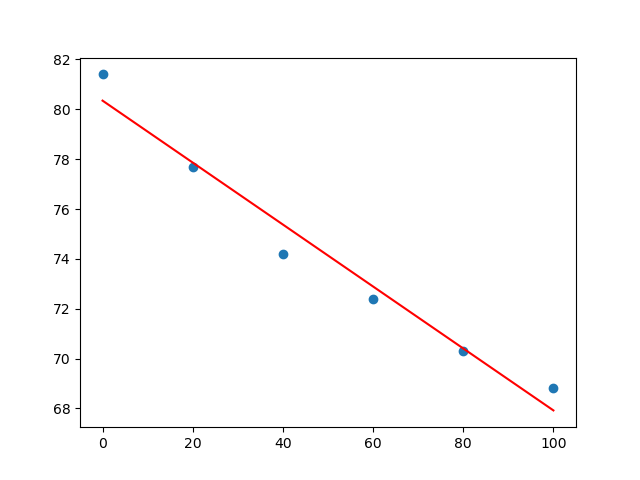
\includegraphics[width=1\linewidth]{Chapter3/graph/python/Figure3-1.png}
    \caption{使用线性拟合结果}
    \label{fig:使用线性拟合结果}
\end{figure}

最后作为扩展演示, 下面是一个使用Legendre多项式进行三次拟合的程序:

\begin{lstlisting}
# 使用Legendre多项式进行三次拟合 Exercise3-3.py
import numpy as np
import matplotlib.pyplot as plt
from scipy.special import legendre
# 示例数据
x = np.array([3.73,5.63,8.67,10.49,13.26,16.74,
19.55,22.19,25.36,28.31,30.83])
y = np.array([21.53,21.43,21.43,21.33,21.22,
20.71,20.20,19.69,18.78,17.76,16.84])
# 进行Legendre拟合
coefficients = np.polynomial.legendre.legfit(x, y, 3)
# 绘制拟合曲线
x_fit = np.arange(3.73,30.83,0.01)
y_fit = np.polynomial.legendre.legval(x_fit, coefficients)
plt.scatter(x,y)
plt.plot(x_fit,y_fit,c="red")
plt.show()
\end{lstlisting}

得到图像如图\ref{fig:使用Legendre多项式进行三次拟合}所示.

\begin{figure}[h]
    \centering
    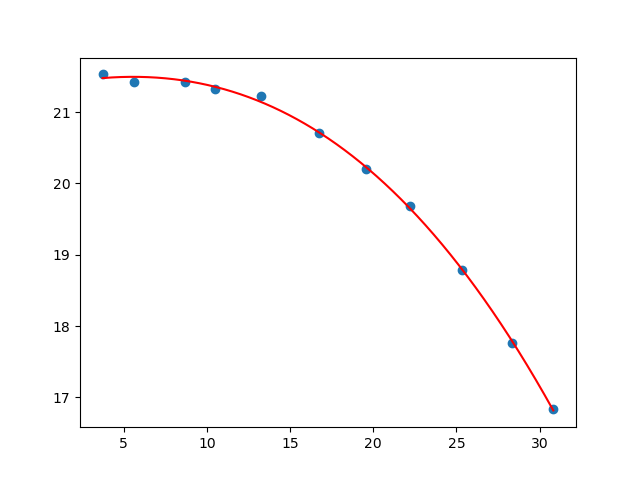
\includegraphics[width=1\linewidth]{Chapter3/graph/python/Figure3-2.png}
    \caption{使用Legendre多项式对一组数据进行三次拟合}
    \label{fig:使用Legendre多项式进行三次拟合}
\end{figure}